% vim: spell spelllang=es:
\documentclass[12pt, oneside]{article}
\usepackage[a4paper, left=2.5cm, right=2.5cm, top=2.5cm, bottom=2.5cm]{geometry}

\usepackage[utf8]{inputenc} % Use unicode
\usepackage[T1]{fontenc}
\usepackage[spanish]{babel} % Names in spanish

%% Bibliography:
%\usepackage{comment}
%\usepackage[
    %backend=biber,
    %style=numeric,
%]{biblatex}
%\DeclareNameAlias{default}{last-first}

%\usepackage{csquotes}       % For bibliography quotations
%\DeclareQuoteAlias{spanish}{catalan}

%\addbibresource{biblio.bib}
%% see:
%% https://www.sharelatex.com/learn/Bibliography_management_in_LaTeX#The_bibliography_file

%\usepackage{datetime} % Customize date
%% \monthyeardate\today gives the date without the day
%\newdateformat{monthyeardate}{%
    %\monthname[\THEMONTH], \THEYEAR}

% For cross references
\usepackage[colorlinks = true]{hyperref}
\usepackage[catalan]{varioref}
%\usepackage{cleveref}
%hyperref configuration so that it doesn't contrast so much colorlinks,
\hypersetup{
   linkcolor={black},
   citecolor={black},
   %linkcolor={red!50!black},
   %citecolor={blue!50!black},
   urlcolor={blue!80!black}
}

\usepackage{mathtools}  % amsmath + more
\usepackage{amsthm}     % Theorem enviroment
\usepackage{amssymb}    % More symbols
\usepackage{amstext}    % Text inside mathenv

\usepackage{relsize}    % Bigger math with mathlarger{___}
\usepackage{nicefrac}   % nice fractions in one line

\usepackage[export]{adjustbox}  % Adjust table size
\usepackage{float}              % Force tables and images position (H and H!)
\usepackage{wrapfig}            % Wrap images like in HTML

\usepackage{tabularx, colortbl, booktabs}    % Better tables
\usepackage{longtable}                      % Multiple page table

% Split cell in lines and more formating options inside table
\usepackage{array, multirow, multicol, makecell}

%\usepackage{subcaption}                     % Subfigures
%\usepackage[framemethod=tikz]{mdframed}     % Custom frames

%\usepackage[bottom]{footmisc} % Footnotes at bottom of page

%\usepackage[alsoload=hep]{siunitx}          % SI units and uncertainties
%\sisetup{locale = FR}                       % Commas and so on for spanish
%\sisetup{separate-uncertainty=true}
%\sisetup{
  %per-mode=fraction,
  %fraction-function=\nicefrac
%}

%\usepackage{tikz}
%%\usetikzlibrary{arrows}
%%\usetikzlibrary{scopes}
%\usetikzlibrary{babel}

%\usepackage{listings}       % For code blocks

%% Custom code highlight
%\definecolor{codegreen}{rgb}{0,0.6,0}
%\definecolor{codegray}{rgb}{0.5,0.5,0.5}
%\definecolor{codepurple}{rgb}{0.58,0,0.82}
%\definecolor{backcolour}{rgb}{0.95,0.95,0.92}
%\definecolor{lightblue}{RGB}{135,206,250}

%\lstdefinestyle{mystyle}{ backgroundcolor=\color{backcolour},
    %commentstyle=\color{codegreen}, keywordstyle=\color{blue},
    %numberstyle=\tiny\color{codegray}, stringstyle=\color{red},
    %identifierstyle=\color{black}, basicstyle=\footnotesize,
    %%breakatwhitespace=false,
    %breaklines=true,
    %%captionpos=b,                    keepspaces=true,
    %numbers=left,                    numbersep=5pt,
    %showspaces=false,
    %%showstringspaces=false, showtabs=false,
    %tabsize=4
%}
%\lstset{style=mystyle}

\newcommand{\whitepage}{
    \clearpage\thispagestyle{empty}\addtocounter{page}{-1} \newpage \clearpage
}

% Add command before appendix session for page numbering: A-1
%\newcommand{\appendixpagenumbering}{
    %\break
    %\pagenumbering{arabic}
    %\renewcommand{\thepage}{\thesection-\arabic{page}}
%}

%% Custom Math operators (functions not in italic in math mode):
%\DeclareMathOperator{\arcsec}{arcsec}
%\DeclareMathOperator{\arccot}{arccot}
%\DeclareMathOperator{\arccsc}{arccsc}
%\DeclareMathOperator{\cis}{cis}


\title{IA Búsqueda local}
\author{%
    Aleix Boné\\
    Alex Herrero\\
    Moisés Balcells\\
}
\date{%
}

% MARIA TERESA ABAD: <mabad@cs.upc.edu>

\begin{document} 
\maketitle


% La documentación deberá incluir:
% La descripción/justificación de la implementación del estado.
% La descripción/justificación de los operadores que habéis elegido...
% La descripción/justificación de las estrategias para hallar la solución inicial.
% La descripción/justificación de las funciones heurísticas.
% Para cada experimento:    
% • Condiciones de cada experimento
% • Resultados del experimento
% • Qué esperabais y qué habéis obtenido    
% • Comparaciones
% • Comentarios adicionales que os parezcan adecuados.
% Comparación entre los resultados obtenidos con Hill Climbing y Simulated Annealing (no olvidéis explicar cómo habéis ajustado los parámetros para este último algoritmo).
% Respuestas razonadas a las preguntas del enunciado.

\section{Implementación del estado}

\section{Operadores que hemos elegido}

\section{Estrategias para hallar la solución inicial}

\section{Funciones heurísticas}

\section{Experimentos}

\subsection{Influencia de los operadores}

\subsection{Influencia de la solución inicial}

\subsection{Parámetros para el simulated annealing}

\subsection{Evolución del tiempo de ejecución para valores crecientes de los parámetros}

\subsubsection{Número de usuarios que piden ficheros}

\begin{tabular}{lrrrr}
\toprule
{} & \multicolumn{2}{l}{time} & \multicolumn{2}{l}{ttt} \\
{} &       media &        std &         media &           std \\
USERS &             &            &               &               \\
\midrule
100   &    0.439545 &   0.344075 &  2.427290e+05 &  20624.964233 \\
200   &    1.782818 &   1.617815 &  4.995559e+05 &  32686.364553 \\
300   &    5.045900 &   0.984051 &  7.645313e+05 &  42743.064831 \\
400   &   10.736700 &   4.973768 &  1.034363e+06 &  51392.984967 \\
500   &   12.388000 &   6.507829 &  1.263917e+06 &  44317.265976 \\
600   &   26.544800 &  12.216475 &  1.543647e+06 &  52970.586044 \\
700   &   34.734900 &  16.169194 &  1.785220e+06 &  67767.572073 \\
800   &   57.239900 &  27.415379 &  2.029594e+06 &  50968.783048 \\
900   &   90.870700 &  26.992538 &  2.305947e+06 &  51138.502401 \\
1000  &  117.450800 &  48.050179 &  2.561704e+06 &  97519.850662 \\
\bottomrule
\end{tabular}


\begin{figure}[H]
\centering
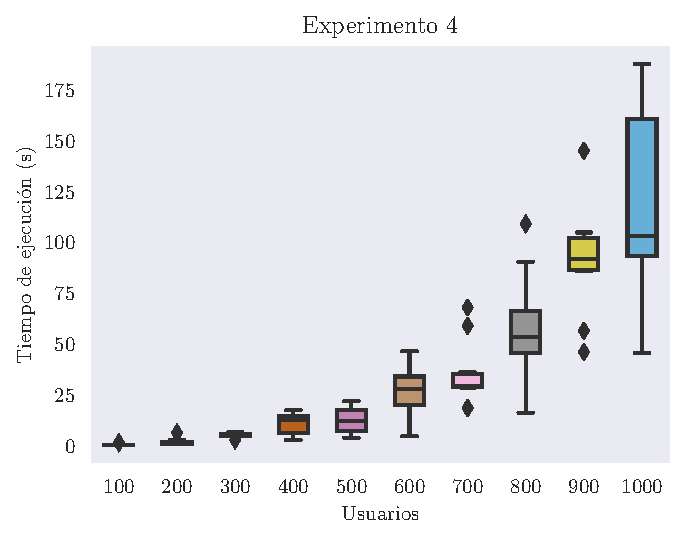
\includegraphics[width=0.8\textwidth]{include/plots/ex4_u_time_bplot.pdf}
\caption{Experimento 7}%
\label{fig:ex7time}
\end{figure}

\subsubsection{Número de servidores (Manteniendo el número de replicaciones)}

\begin{tabular}{lrrrr}
\toprule
{} & \multicolumn{2}{l}{time} & \multicolumn{2}{l}{ttt} \\
{} &     media &       std &          media &           std \\
NSERV &           &           &                &               \\
\midrule
50    &  4.795824 &  2.562619 &  535961.313725 &  54996.663938 \\
100   &  3.693740 &  1.447718 &  551418.460000 &  36156.093438 \\
150   &  3.343780 &  1.184884 &  545857.920000 &  33942.202363 \\
200   &  2.875980 &  1.162004 &  537334.680000 &  31389.152814 \\
250   &  2.675720 &  0.991247 &  522625.080000 &  36122.916802 \\
300   &  2.281000 &  0.777080 &  519116.800000 &  26411.948652 \\
350   &  2.326820 &  0.899757 &  524597.420000 &  25465.987602 \\
400   &  1.843920 &  0.842095 &  508675.920000 &  29198.579187 \\
450   &  1.869560 &  0.764063 &  510638.680000 &  27791.058100 \\
500   &  1.710100 &  0.580861 &  501650.940000 &  22723.234969 \\
550   &  1.834040 &  0.760056 &  502337.700000 &  21553.327865 \\
600   &  1.497540 &  0.524096 &  506234.960000 &  25396.663981 \\
650   &  1.707580 &  0.588698 &  504194.120000 &  31568.463555 \\
700   &  1.216540 &  0.444400 &  498697.960000 &  21463.111941 \\
750   &  1.368400 &  0.532025 &  498214.900000 &  24553.367374 \\
800   &  1.322060 &  0.544356 &  497294.800000 &  25736.299261 \\
850   &  1.266100 &  0.434882 &  495370.360000 &  26499.868047 \\
900   &  1.236180 &  0.580456 &  502435.000000 &  27949.777197 \\
950   &  1.079920 &  0.439555 &  498911.180000 &  21217.998063 \\
1000  &  1.134480 &  0.433452 &  496641.200000 &  21384.378762 \\
\bottomrule
\end{tabular}


\subsection{Diferencia entre Tiempo total de transmisión y tiempo para hallar la solución (Hill Climbing)}

\subsection{Diferencia entre Tiempo total de transmisión y tiempo para hallar la solución (Simulated Annealing)}

\subsection{Influencia del número de replicaciones de los ficheros}

\begin{tabular}{lrrrr}
\toprule
\multirow{2}{*}{NREP} & \multicolumn{2}{c}{$T_{ej}$} & \multicolumn{2}{c}{TTT} \\
{} &  \makecell{Media} &       \makecell{std}           &      \makecell{Media} & \makecell{std}           \\
\midrule
5    &  1.01077 &  0.332965 &  541711.65 &  34079.558824 \\
10   &  1.43681 &  0.480345 &  342630.67 &  20683.481933 \\
15   &  1.96248 &  0.807076 &  260552.10 &  19601.194839 \\
20   &  2.16906 &  0.928984 &  215671.28 &  16023.596047 \\
25   &  2.62371 &  1.245368 &  191069.57 &  14962.044912 \\
\bottomrule
\end{tabular}


\begin{figure}[H]
\centering
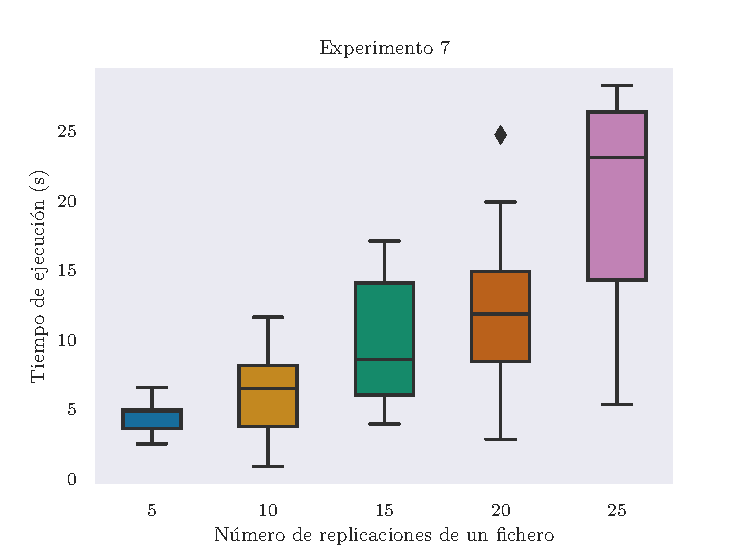
\includegraphics[width=0.8\textwidth]{include/plots/ex7_time_bplot.pdf}
\caption{Experimento 7}%
\label{fig:ex7time}
\end{figure}

\begin{figure}[H]
\centering
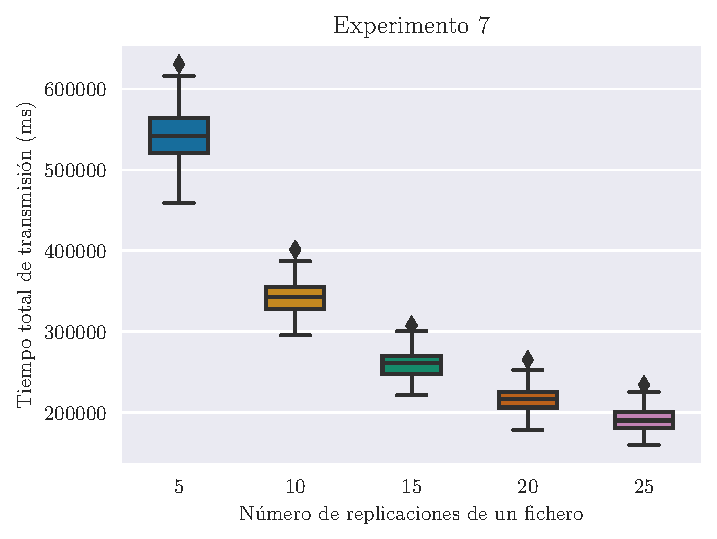
\includegraphics[width=0.8\textwidth]{include/plots/ex7_ttt_bplot.pdf}
\caption{Experimento 7}%
\label{fig:ex7ttt}
\end{figure}

\subsection{Conclusión de los experimentos}
    
    
    
\end{document}